\documentclass[../../compsys.tex]{subfiles}
\begin{document}
\chapter{Introduction to CPU Scheduling}
\vfill
\section{The Need for Scheduling}
In modern computing systems, physical resources are limited, necessitating efficient methods to share these resources among multiple processes and threads. CPU scheduling is a fundamental concept in operating systems that addresses how to allocate processor time among competing tasks.

\subsection{Resource Sharing Approaches}
There are two main approaches to achieve resource sharing in computing systems:

\begin{itemize}
    \item[-] \textbf{Time Sharing} — Running one task at a time and rapidly switching among multiple tasks. In this approach, each task gets exclusive access to the resource for a limited time period.
    \item[-] \textbf{Space Sharing} — Dividing the available resource so that each task receives a portion of the total space simultaneously.
\end{itemize}

\newpage
\section{Fundamentals of CPU Scheduling}
The primary goal of CPU scheduling is to create the illusion that each thread has exclusive use of the processor, while in reality, the CPU is being shared among multiple threads. This illusion is maintained through efficient time sharing of the CPU resource.
  
\subsection{Thread Types and Scheduling}
Threads can be categorized based on their operation patterns:
\begin{itemize}
    \item[-] \textbf{CPU-bound threads}: Perform computations with minimal I/O calls (e.g., calculating Fibonacci numbers)
    \item[-] \textbf{I/O-bound threads}: Frequently make I/O calls (e.g., reading from disk, waiting for network)
\end{itemize}

\subsection{Thread States}
Thread states represent the different operational conditions a thread can be in during its lifecycle.
\begin{minipage}{0.45\textwidth}
    \begin{itemize}
        \item[-] \textbf{Running}: The thread is currently being executed by the CPU.
        \item[-] \textbf{Ready}: The thread is waiting to be executed by the CPU.
        \item[-] \textbf{Blocked}: The thread is waiting for an event to occur (e.g., I/O completion, message arrival).
    \end{itemize}
\end{minipage}
\hfill
\begin{minipage}{0.45\textwidth}
    \centering
    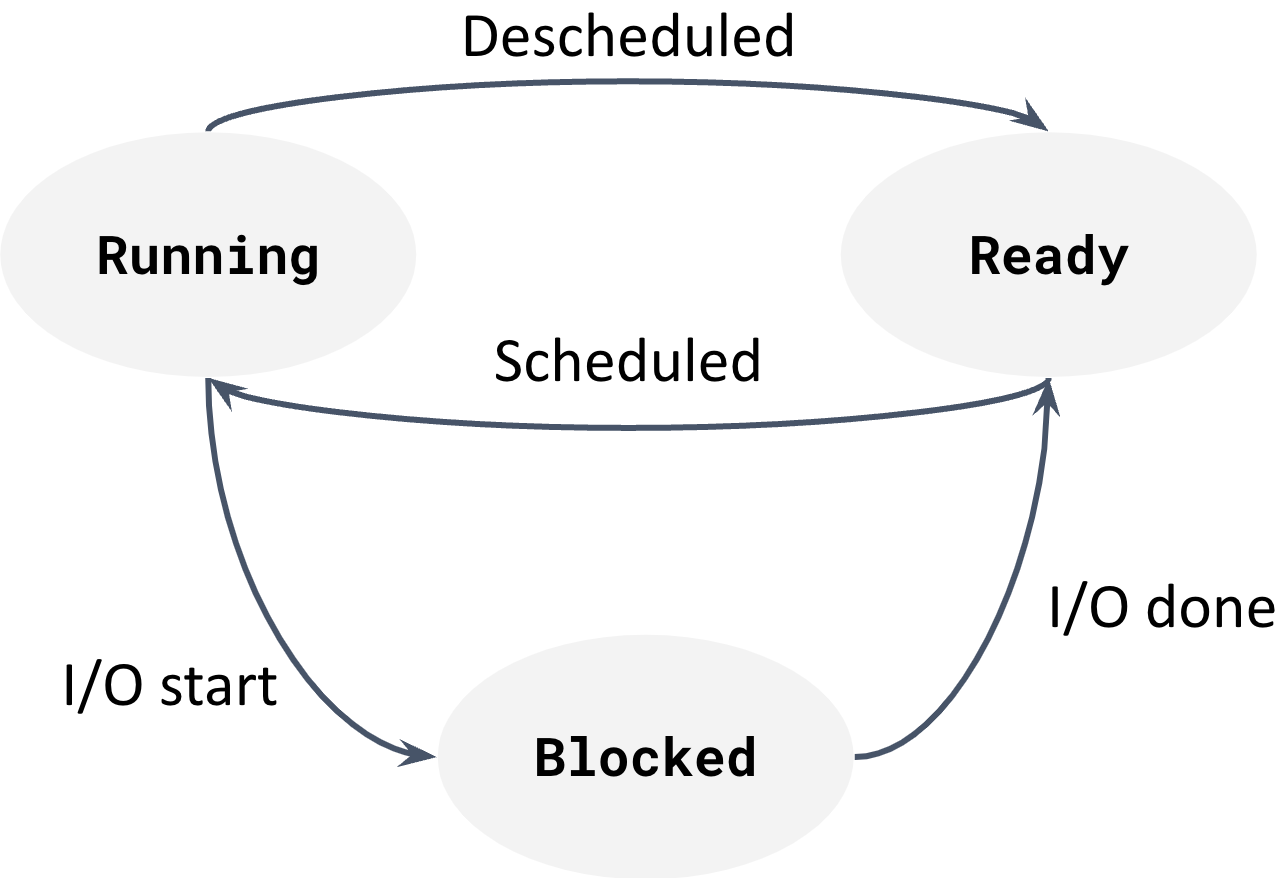
\includegraphics[width=0.9\textwidth]{images/thread_states.png}
\end{minipage}


\subsection{Role of the Operating System Scheduler}
The operating system's scheduler is responsible for:
\begin{itemize}
    \item[-] Maintaining a list of all threads in the system
    \item[-] Tracking each thread's state (running, ready, blocked, etc.)
    \item[-] Selecting which thread to run next according to a defined scheduling policy
    \item[-] Managing context switches to give each thread its turn on the CPU
\end{itemize}

\subsection{Reasons for Thread Scheduling}
The operating system may need to schedule a new thread for various reasons:
\begin{itemize}
    \item[-] The current thread has completed execution or terminated (e.g., due to invalid operations)
    \item[-] The thread has made a system call (e.g., I/O operation) and must wait for its completion
    \item[-] The OS scheduler has determined another thread should run (e.g., time slice expired)
    \item[-] Other threads with higher priority are present in the ready queue
\end{itemize}

\subsection{Context Switching}
Context switching is the process of saving the state of a currently running thread and loading the state of another thread. This mechanism enables time-sharing of the CPU resource.\\[5px]
\begin{minipage}[htp]{0.45\textwidth}
    The OS performs the following operations during a context switch:
    \begin{enumerate}
        \item Saves the running thread's execution state (registers, program counter, etc.) in memory
        \item Selects the next thread to run according to the scheduling policy
        \item Restores the execution state of the selected thread
        \item Passes control to the thread using a return-from-trap mechanism
    \end{enumerate}
\end{minipage}
\hfill
\begin{minipage}[htp]{0.45\textwidth}
    \centering
    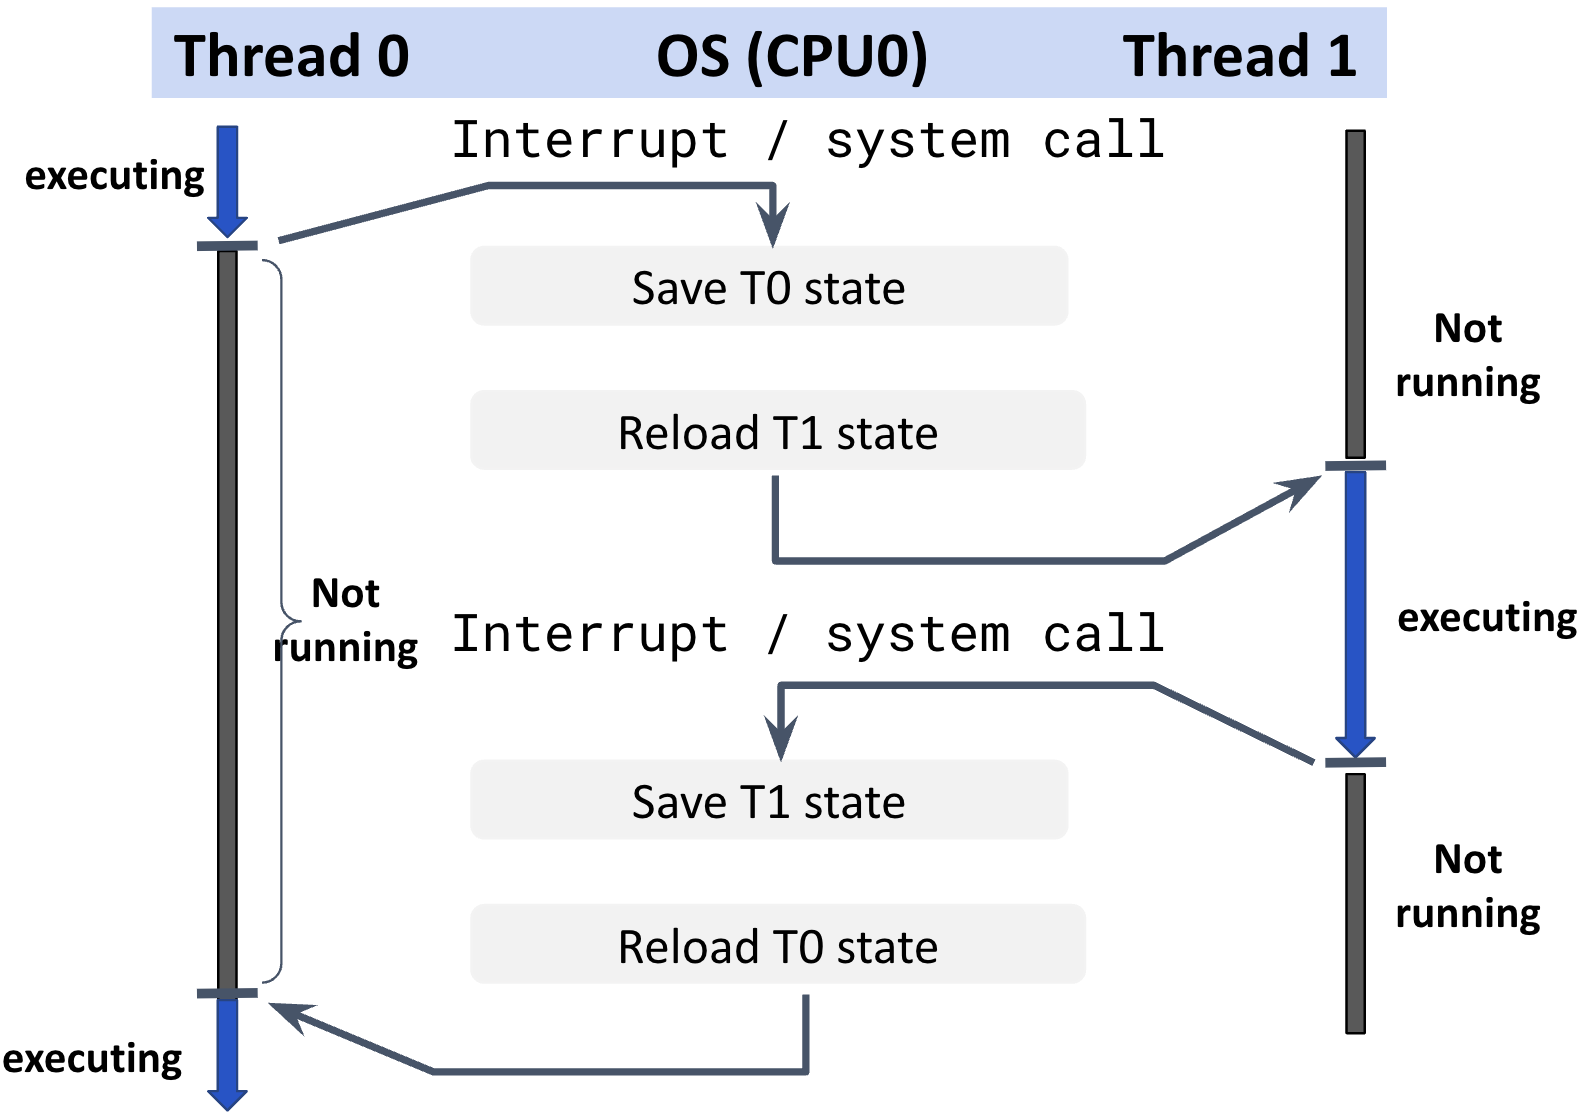
\includegraphics[width=\textwidth]{images/context_switch.png}
\end{minipage}


\subsection{Handling Misbehaving Threads}
A critical challenge in operating systems is managing threads that may:

    \begin{minipage}[htp]{0.45\textwidth}
        \begin{itemize}
            \item[-] Refuse to give up CPU control on their own
            \item[-] Run in infinite loops without performing I/O operations
            \item[-] Attempt to monopolize system resources
        \end{itemize}
    \end{minipage}
    \hfill
    \begin{minipage}[htp]{0.45\textwidth}
        \centering
        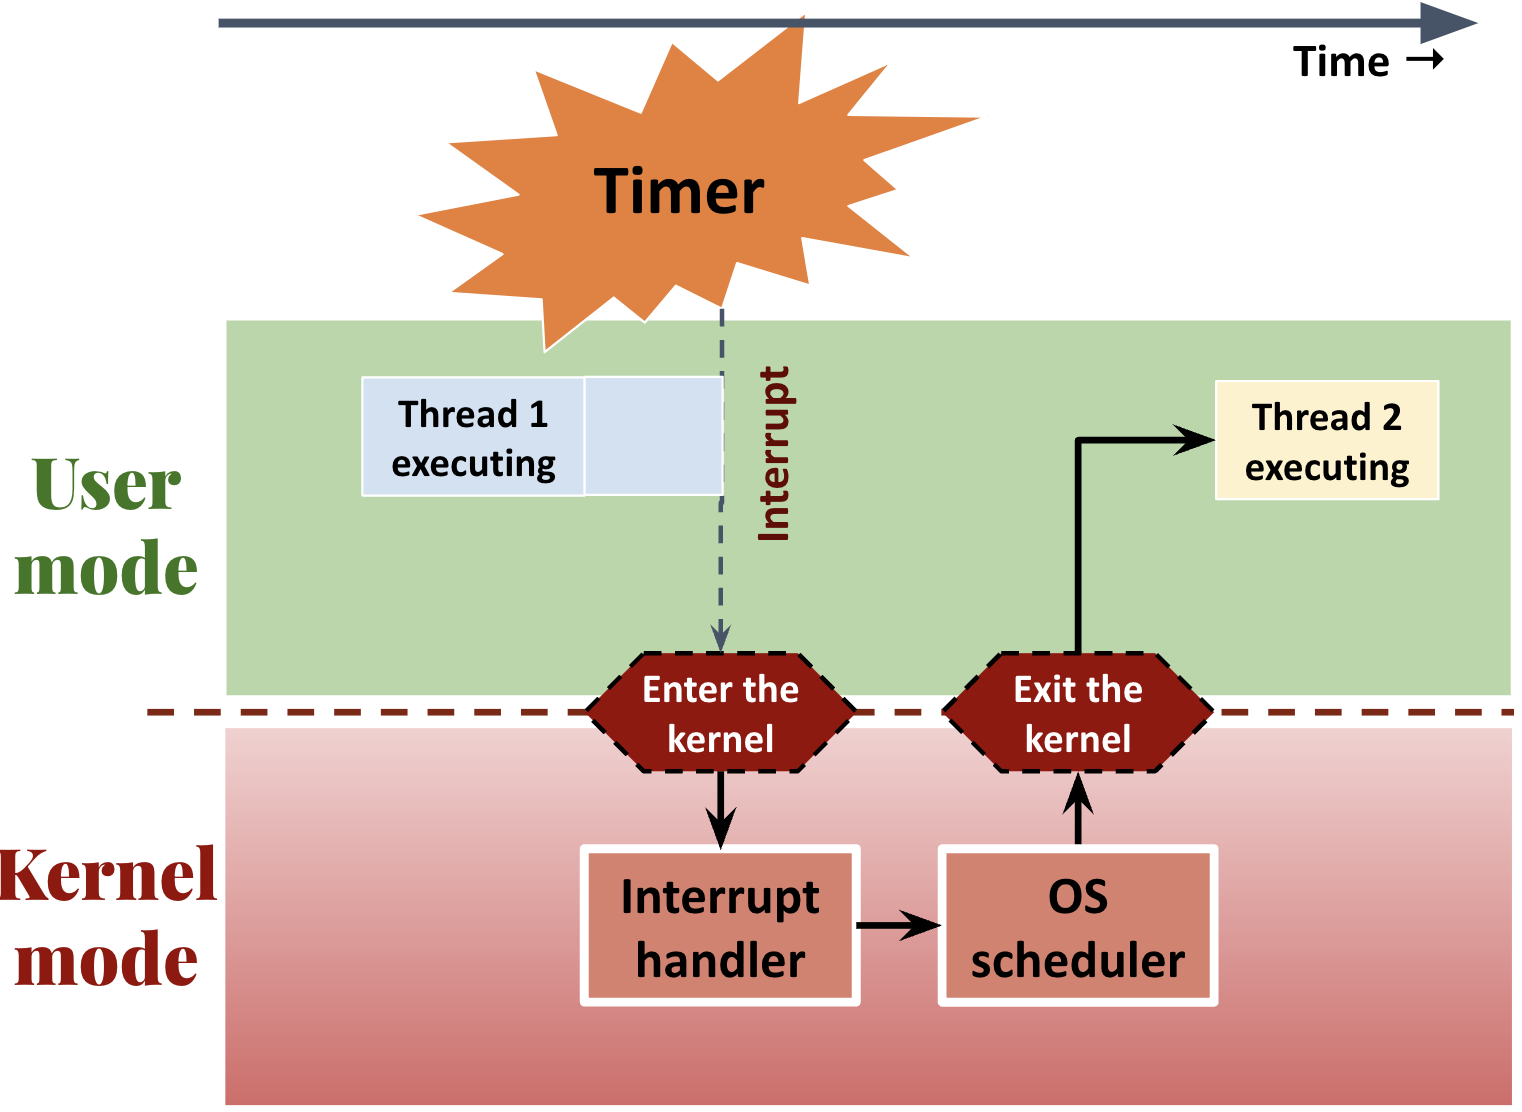
\includegraphics[width=0.95\textwidth]{images/misbehaving_threads.png}
\end{minipage}\\[5px]

To address this challenge, operating systems implement preemptive scheduling using hardware timer interrupts.
The process works as follows:
\begin{enumerate}
    \item The OS sets a hardware timer before scheduling a thread
    \item When the timer expires, the CPU is interrupted
    \item The current thread is suspended and the system switches to kernel mode
    \item The interrupt handler invokes the OS scheduler
    \item The scheduler selects the next thread and performs a context switch
\end{enumerate}

This mechanism ensures that no single thread can monopolize the CPU indefinitely, maintaining fairness in resource allocation.

\newpage
\section{Scheduling Policies}
The scheduling policy is a key component of the operating system that determines which thread should run next. When a system has multiple threads competing for CPU time, the policy establishes the order in which threads execute.

\subsection{Scheduling Metrics}
To evaluate and compare different scheduling policies, we use performance metrics that quantify system behavior. Two fundamental metrics are:

\begin{enumerate}
    \item \textbf{CPU Utilization}: The fraction of time the CPU is executing thread code.
    \begin{itemize}
        \item[-] \textbf{Goal}: Maximize CPU utilization (keep the CPU as busy as possible)
        \item[-] Measured as a percentage from 0\% (idle) to 100\% (fully utilized)
    \end{itemize}
    
    \item \textbf{Turnaround Time}: The total time from a thread's arrival to its completion.
    \begin{itemize}
        \item[-] \textbf{Goal}: Minimize turnaround time for better system responsiveness
        \item[-] Mathematical definition: $T_{turn around} = T_{completion} - T_{arrival}$
    \end{itemize}
\end{enumerate}

\subsection{First In, First Out (FIFO)}
FIFO (also known as First Come, First Served) is the simplest scheduling algorithm where threads are executed in the order they arrive in the ready queue.
\subsubsection{FIFO with Equal Run Times}
Consider a scenario with three threads (A, B, C) that arrive simultaneously and each requires 10 seconds of CPU time \\[5px]
\textbf{Assumptions:}\\[5px]
\begin{minipage}[htp]{0.5\textwidth}
 - Each thread runs for the same time (10s) \\[5px]
 - All threads arrive at the same time ($T_{arrival} = 0$) \\[5px]
 - Each thread runs to completion \\[5px]
 - Run-time of threads is known in advance \\[5px]
\end{minipage}
\hfill
\begin{minipage}[htp]{0.5\textwidth}
    \centering
    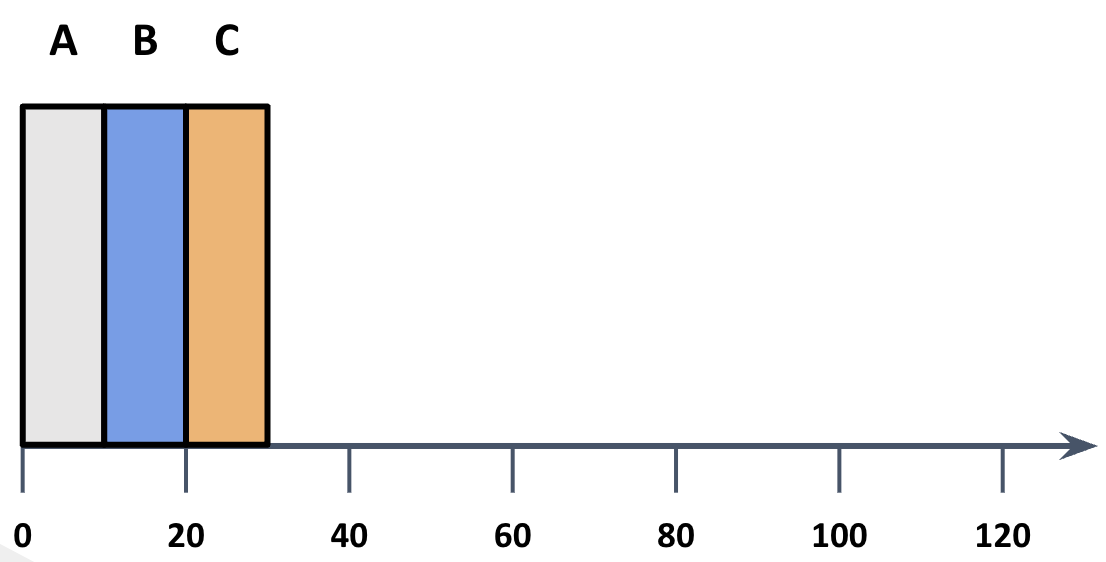
\includegraphics[width=0.95\textwidth]{images/fifo.png}
\end{minipage}\\[5px]
\textbf{Calculations:}
\begin{align*}
    T_{arrival} &= 0 \\
    T_{completion}(A) &= 10 \\
    T_{completion}(B) &= 20 \\
    T_{completion}(C) &= 30
\end{align*}

\textbf{Average turnaround time} = $\frac{10 + 20 + 30}{3} = 20$ seconds
\subsubsection{FIFO with Varied Run Times}
Now consider a scenario where thread A requires much more CPU time than the others:\\[5px]
\textbf{Assumptions:}\\[5px]
\begin{minipage}[htp]{0.5\textwidth}
        - Threads have different run times \\(A: 100s, B: 10s, C: 10s) \\[5px]
        - All threads arrive at the same time ($T_{arrival} = 0$) \\[5px]
        - Each thread runs to completion \\[5px]
        - Run-time of threads is known in advance \\[5px]
\end{minipage}
\hfill
\begin{minipage}[htp]{0.5\textwidth}
    \centering
    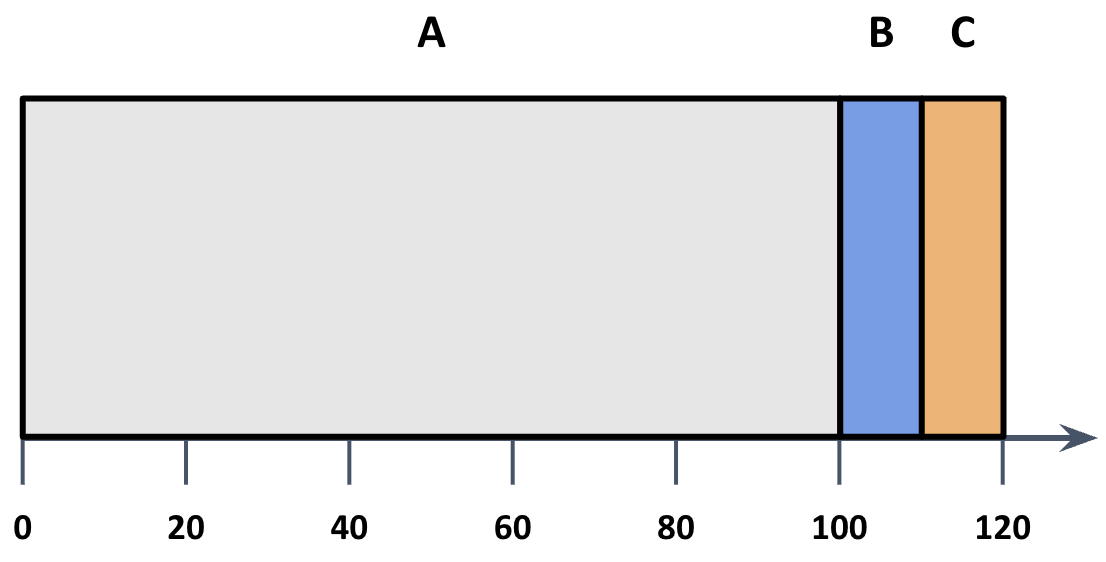
\includegraphics[width=0.95\textwidth]{images/fifo_challenge.png}
\end{minipage}\\[8px]

\textbf{Calculations}
\begin{align*}
    T_{arrival} &= 0 \\
    T_{completion}(A) &= 100 \\
    T_{completion}(B) &= 110 \\
    T_{completion}(C) &= 120
\end{align*}
\textbf{Average turnaround time} = $\frac{100 + 110 + 120}{3} = 110$ seconds \\[3px]
In FIFO scheduling, long-running threads can significantly delay shorter threads, causing poor average turnaround times. This is known as the "convoy effect" and represents a major limitation of the FIFO scheduling policy\\[3px]
\textit{basically, the classic - someone in a supermarket queue is buying a lot of stuff and you're waiting for them to finish even though you have less items than them}
\subsection{Shortest Job First (SJF)}
Choose ready threads with shortest running time\\
\textbf{Assumptions:}\\[5px]
\begin{minipage}[htp]{0.5\textwidth}   
Assume 3 threads (A, B, C): A runs for 100 seconds, while B and C run 10 seconds
\end{minipage}
\hfill
\begin{minipage}[htp]{0.45\textwidth}
    \centering
    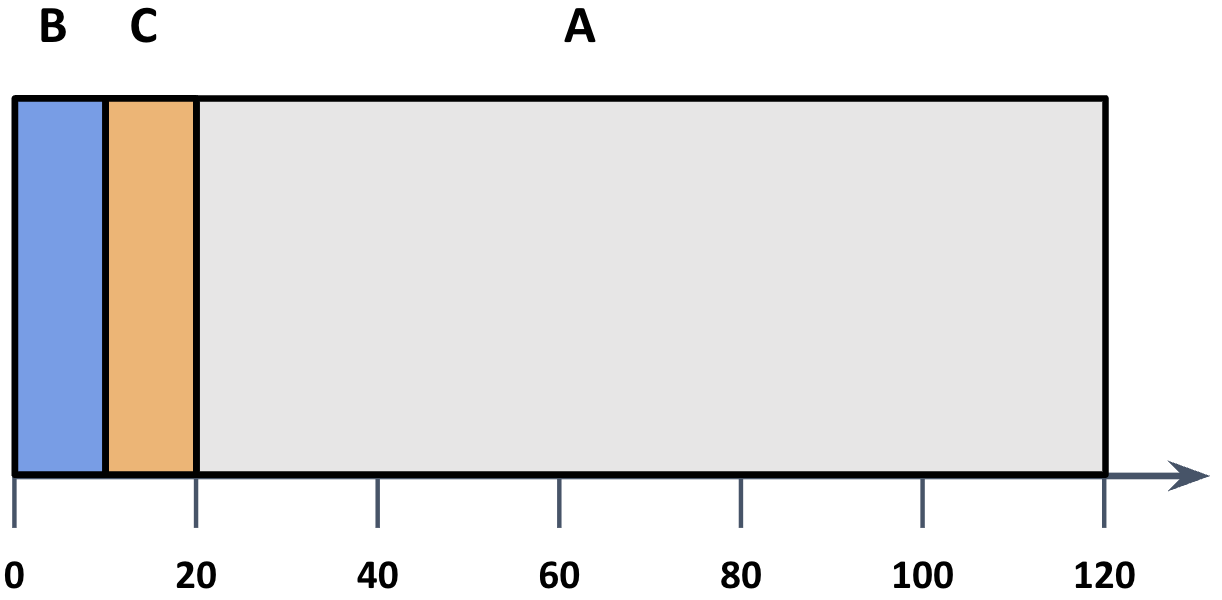
\includegraphics[width=1\textwidth]{images/sjf.png}
\end{minipage}\\[5px]
\textbf{Calculations:}\\[5px]
\begin{align*}
    T_{arrival} &= 0 \\
    T_{completion}(A) &= 120 \\
    T_{completion}(B) &= 10 \\
    T_{completion}(C) &= 20
\end{align*}
\textbf{Average turnaround time} = $\frac{120 + 10 + 20}{3} = 50$ seconds \\[3px]
Turnaround time improves by almost 50\%
\subsubsection{Issue with SJF}
A runs for 100 seconds, while B and C run 10 seconds
\textbf{Assumptions:}\\[5px]
\begin{minipage}[htp]{0.45\textwidth}
    \begin{itemize}
        \item[-] Threads do not need to run for same time
        \item[-] Threads do not need to arrive at same time
        \item[-] Each thread runs to completion
        \item[-] Run-time of threads is known
    \end{itemize}
\end{minipage}
\hfill
\begin{minipage}[htp]{0.45\textwidth}
    \centering
    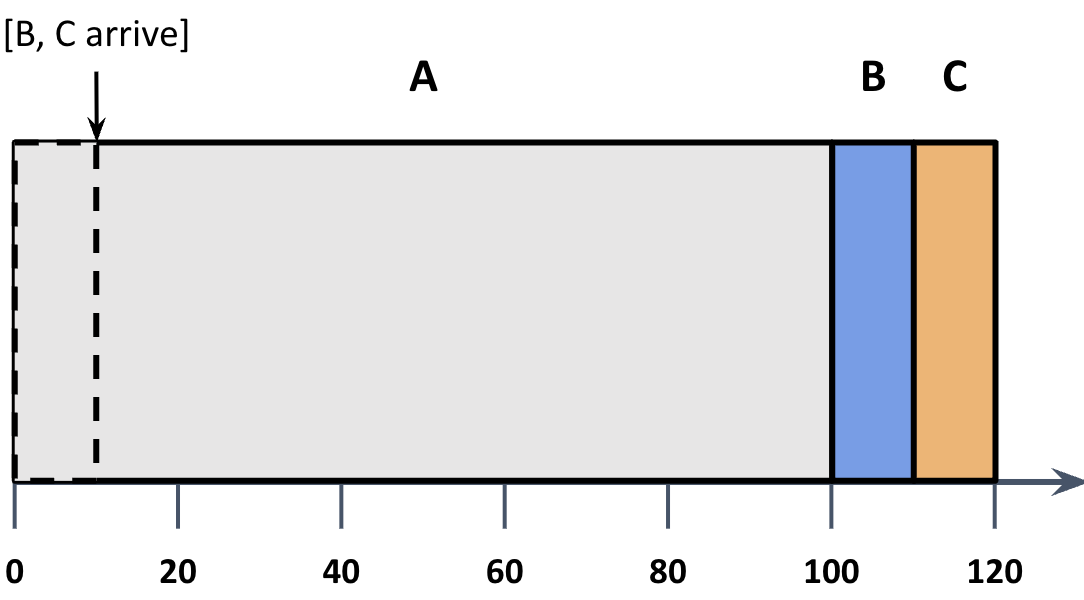
\includegraphics[width=0.95\textwidth]{images/sjf_issue.png}
\end{minipage}\\[5px]
\textbf{Calculations:}\\[5px]
\begin{align*}
   T_{arrival}(A) &= 0 \\
   T_{arrival}(B) &= T_{arrival}(C) = 10 \\
   T_{completion}(A) &= 100 \\
   T_{completion}(B) &= 110 \\
   T_{completion}(C) &= 120
\end{align*}
\textbf{Average turnaround time} = $\frac{100 + (110 - 10) + (120 - 10)}{3} = 103.3$\\[5px]
\textbf{Remark: } Long running threads cannot be interrupted, leading to convoy effect
\subsection{Polite vs. forced scheduling}
\textbf{Non-preemptive Scheduling:}\\[5px]
\begin{itemize}
    \item[-] Previous schedulers (FIFO, SJF) are non-preemptive
    \item[-] Only switch to other threads once the current thread finishes its whole execution (run-to-completion)
    \item[-] OS has no control on a thread's completion time
\end{itemize}

\textbf{Preemptive Scheduling:}\\[5px]
\begin{itemize}
    \item[-] Stops the execution of the current thread and switches to other ready thread forcibly
    \item[-] OS avoids CPU monopolization and maintains control (thread create/destroy, timer interrupts)
    \item[-] \textbf{This removes the assumption that each job runs to completion}
\end{itemize}
\newpage
\subsection{Shortest Time to Completion First (STCF)}
STCF extends the SJF by adding preemption\\
\textbf{Assumptions:}\\[5px]
\begin{minipage}[htp]{0.45\textwidth}
\begin{itemize}
    \item[-] Any time a new thread is created:
    \item[-] STCF scheduler determines which of the remaining jobs (including new job) has the least time left
    \item[-] STCF then schedules the shortest job first
\end{itemize}
\end{minipage}
\hfill
\begin{minipage}[htp]{0.45\textwidth}
    \centering
    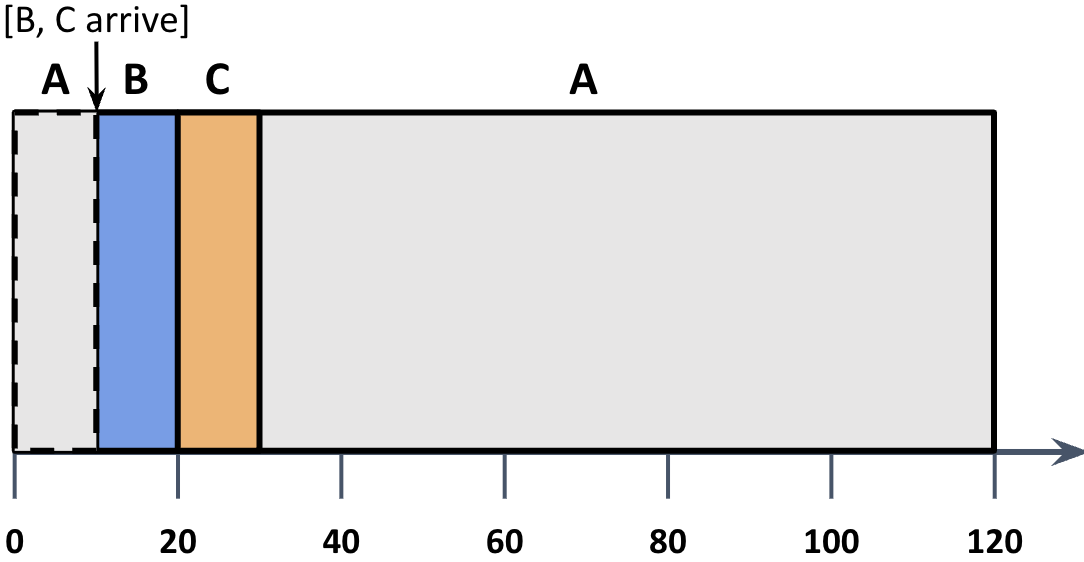
\includegraphics[width=0.95\textwidth]{images/stcf.png}
\end{minipage}\\[5px]
\textbf{Calculations:}\\[5px]
\begin{align*}
    T_{arrival}(A) &= 0 \\
    T_{arrival}(B) &= T_{arrival}(C) = 10 \\
    T_{turnaround}(A) &= 120 \\
    T_{turnaround}(B) &= (20 - 10) = 10 \\
    T_{turnaround}(C) &= (30 - 10) = 20
\end{align*}
\textbf{Average turnaround time} = $\frac{120 + 10 + 20}{3} = 50$ seconds \\[3px]

\textbf{Remark:} Reschedule when new threads arrive, prioritize short running threads
\subsection{New Metric  - Response Time}
\textbf{Previous metrics:}\\[5px]
\begin{itemize}
    \item[-] Focused only on turnaround time (i.e., completing the threads' execution as fast as possible)
    \item[-] Turnaround time is important for batch jobs (non-interactive tasks)
\end{itemize}

\textbf{New metric:}\\[5px]
\begin{itemize}
    \item[-] Response time became equally important
    \item[-] Defined as how long it takes until a thread is scheduled for the first time
\end{itemize}
\subsubsection{STCF with Response Time}
For example, for the STCF\\
\textbf{Response time:} Time from when the job arrives in the system to the first time it is scheduled:\\[3px]
$T_{response} = T_{firstrun} - T_{arrival}$\\[5px]

\textbf{Calculations:}\\[5px]
\begin{align*}
    T_{arrival}(A) &= 0 \\
    T_{arrival}(B) &= T_{arrival}(C) = 10 \\
    T_{response}(A) &= (0 - 0) = 0 \\
    T_{response}(B) &= (10 - 10) = 0 \\
    T_{response}(C) &= (20 - 10) = 10
\end{align*}

\textbf{Average response time} = $\frac{0 + 0 + 10}{3} = 3.3$ seconds\\[5px]
\subsubsection{STCF is still not perfect}
\textbf{Prior scheduling policies are not good for response time:}\\[5px]
Consider 3 jobs arrive at T=0 with same running time, the third job has to wait for the previous two jobs before getting scheduled!\\
This is great for turnaround time, but bad for interactivity.\\
Another way to think: typing on a keyboard and waiting \textbf{seconds} for the character to show up on the screen...
\subsection{Round Robin Scheduling}
Instead of running threads to completion, RR schedules a thread for a fixed interval (or a time-slice) and then switches to the next thread
Alternate ready threads every fixed-length time slice. 
\subsubsection{Round Robin vs STCF}
Threads A, B, and C run for 5 seconds each and arrive at time 0, $T_{arrival} = 0$\\[5px]

\begin{minipage}[htp]{0.5\textwidth}
    \begin{itemize}
        \item[-] In SJF, each thread runs to completion before running another
        \item[-] Average response time = (0 + 5 + 10) / 3 = 5
        \item[-] Average turnaround time = (5 + 10 + 15)  / 3 = 10
    \end{itemize}
    \begin{center}
        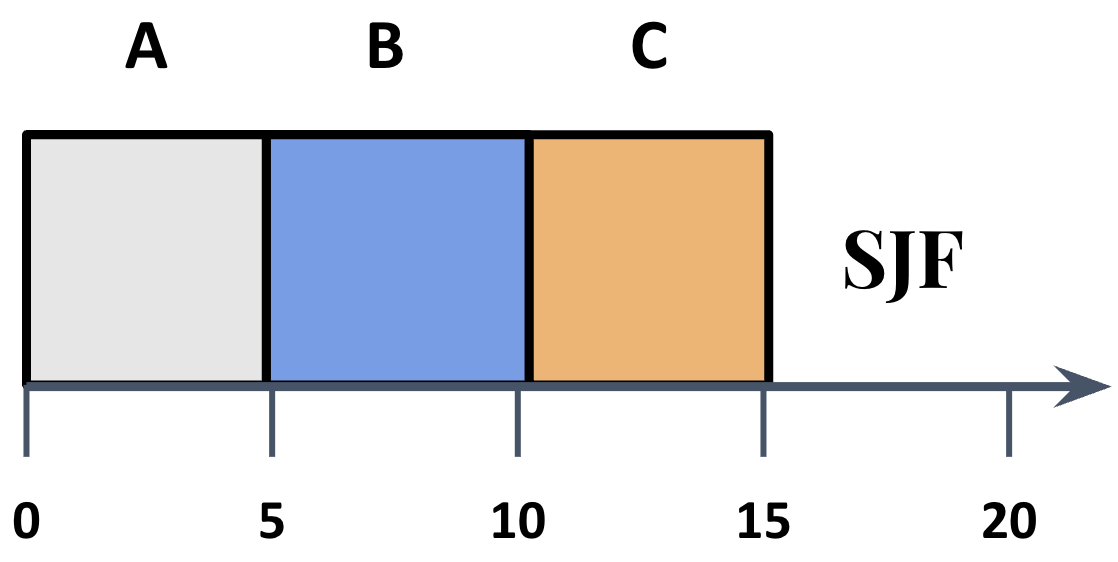
\includegraphics[width=0.75\textwidth]{images/vs_sjf.png}
    \end{center}
\end{minipage}
\hfill
\begin{minipage}[htp]{0.5\textwidth}
    \begin{itemize}
        \item[-] In RR, time slice is 1 second and it will run each thread every second
        \item[-] Average response time = (0 + 1 + 2) / 3 = 1
        \item[-] Average turnaround time = (13 + 14 + 15) / 3 = 14
    \end{itemize}
    \begin{center}
        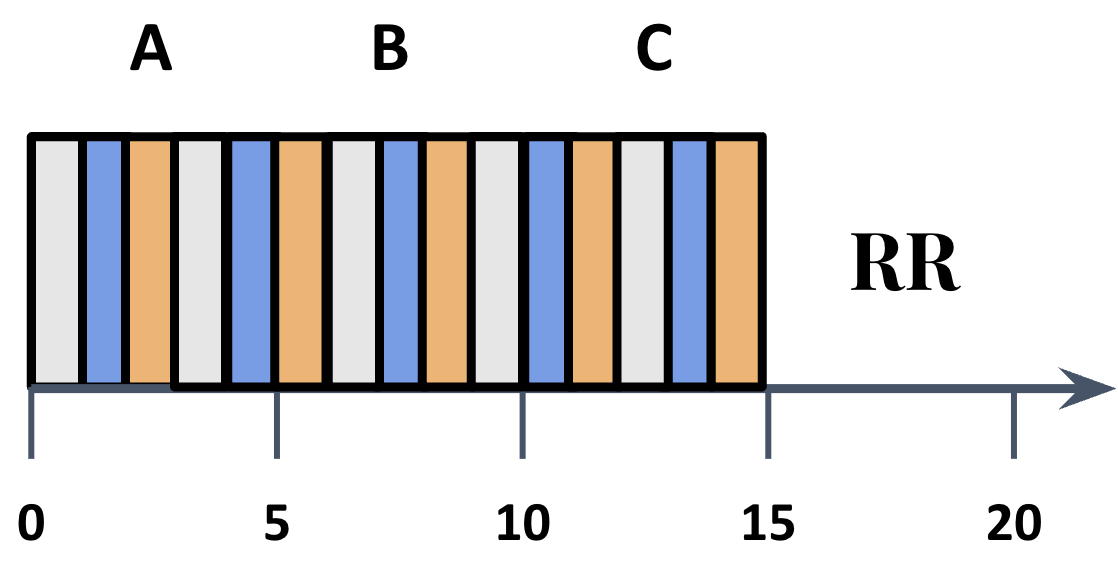
\includegraphics[width=0.75\textwidth]{images/vs_rr.png}
    \end{center}
\end{minipage}\\
\textbf{Remark: Responsiveness increases turnaround (for equally long running threads)}
\subsection{IO Request Scheduling}
In operating systems, we need to consider how IO operations affect CPU scheduling. Let's examine a simple example:

Assume we have two threads (A and B):
\begin{itemize}
    \item Thread A needs 40 ms of CPU time and makes 3 IO requests of 10 ms each
    \item Thread B needs 40 ms of CPU time and makes no IO requests
    \item Thread A issues an IO request every 10 ms of CPU time
\end{itemize}

When thread A issues IO requests, the CPU is not utilized efficiently if the scheduler doesn't account for this behavior.

\subsubsection{Scheduling with IO Awareness}
\textbf{Question: } For a Shortest Time-to-Completion First (STCF) scheduler, how should we handle thread A's 4 sub-jobs (10 ms each) versus thread B's single 40 ms job?

\textbf{Answer: } A better approach is for the scheduler to account for both IO and CPU time to improve resource utilization:
\begin{itemize}
    \item[-] Treat each of A's 10 ms segments as independent sub-jobs
    \item[-] Consider B as a whole 40 ms job
    \item[-] STCF chooses A's first sub-job (10 ms) and then schedules B
    \item[-] When A's next sub-job becomes ready, the scheduler preempts B
    \item[-] While A waits for IO completion, B can run on the CPU
    \item[-] This leads to better CPU utilization through overlapping CPU and IO operations
\end{itemize}

\subsection{Multi-level Queue Scheduling (MLFQ)}
\subsubsection{The Scheduling Challenge}
A general-purpose scheduler must support different types of threads:
\begin{itemize}
    \item \textbf{Batch-processing threads:} Long-running background processes that need lots of CPU time but where response time is not critical
    \item \textbf{Interactive threads:} Foreground processes that require low latency and run in short bursts (need frequent but small amounts of CPU time)
\end{itemize}

\subsubsection{MLFQ Approach}
MLFQ aims to optimize for both types of threads:
\begin{itemize}
    \item First, it tries to optimize turnaround time (important for batch threads)
    \item Then, it minimizes response time for better interactivity
\end{itemize}

The challenge is that the scheduler doesn't know the total runtime of a thread in advance (which would be needed for SJF or STCF). The insight of MLFQ is to use past behavior as a predictor for future behavior.

\subsubsection{MLFQ Implementation}
MLFQ uses multiple levels of Round Robin queues:
\begin{itemize}
    \item Each level has a different priority
    \item Higher levels preempt lower levels
    \item Higher levels have shorter time slices
    \item Lower levels have longer time slices
\end{itemize}

\subsubsection{MLFQ Rules}
The scheduler follows these rules to adjust priorities dynamically:
\begin{enumerate}
    \item If priority(A) $>$ priority(B), then A runs
    \item If priority(A) = priority(B), then A and B run in Round Robin
    \item All threads start at the highest priority level
    \item If a thread uses its entire time slice, the scheduler lowers its priority
    \item Periodically, all threads are moved back to the highest priority queue (called "priority boosting")
\end{enumerate}

The periodic priority boosting (rule 5) prevents starvation, which could happen when multiple IO-bound threads at high priority might prevent a CPU-bound thread at low priority from ever running.

\begin{example}[MLFQ in Action]
\leavevmode
\upshape
Let's see how MLFQ works with a concrete example. Assume we have a system with three priority queues (Q2, Q1, Q0), where Q2 is the highest priority:
\begin{minipage}[htp]{0.45\textwidth}
\begin{itemize}
    \item[-] Each queue uses Round Robin scheduling
    \item[-] Time slice for Q2 = 10 ms, Q1 = 10 ms, Q0 = 30 ms
    \item[-] Priority boost happens every 50 ms
\end{itemize}
\end{minipage}
\hfill
\begin{minipage}[htp]{0.45\textwidth}
    \begin{center}
        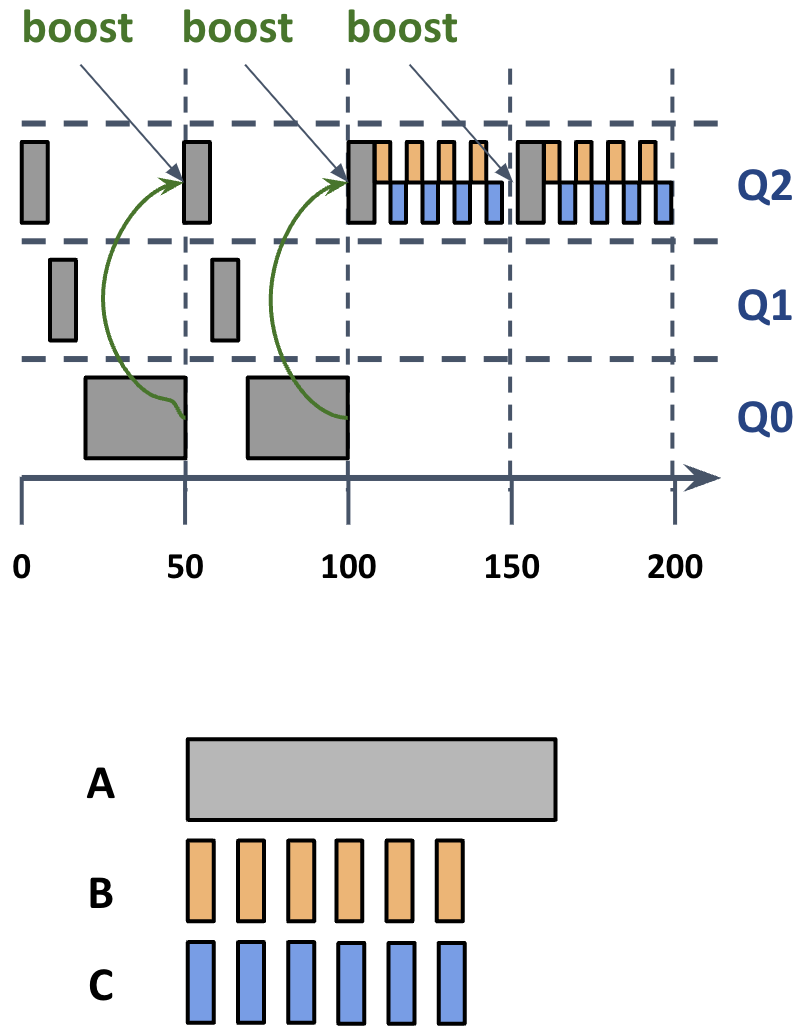
\includegraphics[width=0.65\textwidth]{images/mlfq_example.png}
    \end{center}
\end{minipage}\\
\textbf{Phase 1: Single CPU-bound process}
\begin{enumerate}
    \item Process A begins in Q2 (highest priority)
    \item A uses its entire 10 ms time slice in Q2 and gets demoted to Q1
    \item A uses its entire 10 ms time slice in Q1 and gets demoted to Q0
    \item A runs in Q0 for 30 ms until the priority boost occurs
    \item After the boost, A returns to Q2 and the cycle repeats
\end{enumerate}

\textbf{Phase 2: Interactive processes arrive}
\begin{enumerate}
    \item After A has been running for 100 ms, processes B and C join the system
    \item All three processes (A, B, C) are now in Q2
    \item A runs for 10 ms and gets demoted to Q1
    \item Now B runs for a short time but issues an IO request before using its full time slice
    \item C also runs briefly before issuing an IO request
    \item Since B and C issue frequent IO requests, they never use their full time slices
    \item B and C therefore remain in Q2, while A continues to be demoted
\end{enumerate}

\textbf{Result:} Interactive processes (B and C) get quick response times by staying in the high-priority queue, while the CPU-intensive process (A) is given fair access through priority boosting. This demonstrates how MLFQ adapts to different process types without requiring advance knowledge of their behavior.
\end{example}
\hrule
\vspace{10px}
Good Luck for the midterm ! 
\end{document}